\section{Analysis of Random Forest Feature Importances}

The feature importance plot from our Random Forest model provides valuable insights into which features are most influential in predicting credit card fraud. Here's a detailed analysis:

\subsection{Most Important Features}
\begin{itemize}
    \item V17 is by far the most important feature, with a relative importance of approximately 0.2 (20\%).
    \item V14 is the second most important, with importance around 0.17 (17\%).
    \item V12 is third, with importance close to 0.14 (14\%).
\end{itemize}

\subsection{Least Important Features}
Many features (V21, V1, V5, V6, V2, V19, V26, Amount, V13, V8, Time, V15, V20, V25, V22, V28, V24, V23, V27) have very low importance, barely visible on the chart.

\subsection{Key Observations}
\begin{itemize}
    \item The 'Amount' feature has surprisingly low importance, suggesting that the transaction amount alone is not a strong predictor of fraud in this model.
    \item 'Time' also has very low importance, indicating that the time of transaction may not be a crucial factor in detecting fraud.
    \item The features are named V1, V2, etc., which suggests they might be derived features or principal components, possibly from a dimensionality reduction technique applied before the Random Forest model.
\end{itemize}

\begin{figure}[h]
    \centering
    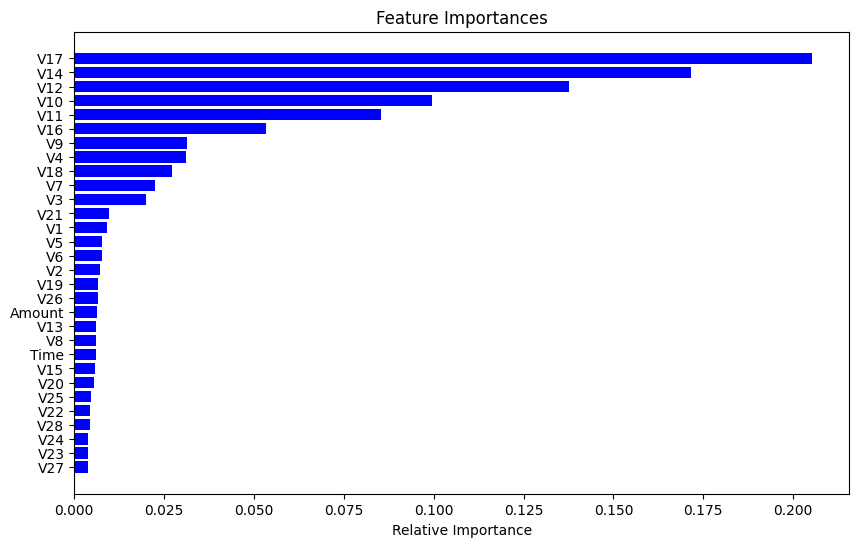
\includegraphics[width=0.8\linewidth]{Random Forest Feature Importances.png}
    \caption{Random Forest Feature Importances}
    \label{fig:Random Forest Feature Importances}
\end{figure}
